\chapter{Data-Driven Coarsening of Finite Elements}
\section{Background}
\subsection{The Finite Element Method}
The finite element method~\citep{ciarlet2002finite} is a way to numerically approximate solutions to partial differential equations.
The function domain $\Omega$ is divided into a finite number of elements $E_k$.
A polynomial function is defined over each element.
These polynomials form a basis for discrete approximations to the solution.

This thesis uses eight-node hexahedron elements defined in $\mathbb{R}^3$
to perform all of the mechanical analysis.
The eight-node hexahedron element is the simplest of the hexahedron family.
It represents continuous functions by trilinearly interpolating function values defined on its eight nodes.
\begin{figure}
\centering
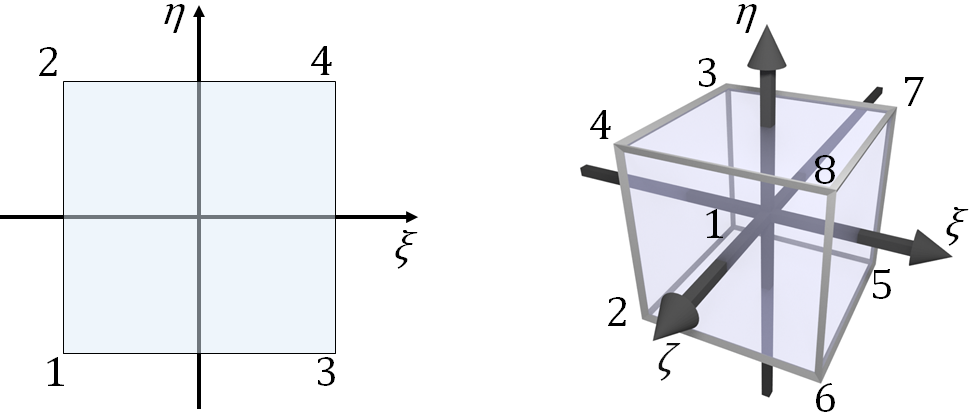
\includegraphics[width=0.8\textwidth]{figs/refEle.png}
\caption{Standard elements for 2D quadrilateral (left) and 3D hexahedral elements.}
\label{fig:standardEle}
\end{figure}
\subsection{Modeling Elastic Objects}

\section{}
